\documentclass[]{BasiliskReportMemo}
\usepackage{AVS}


\newcommand{\submiterInstitute}{Autonomous Vehicle Simulation (AVS) Laboratory,\\ University of Colorado}

\newcommand{\ModuleName}{imu\_sensor}
\newcommand{\subject}{Testing IMU Sensor Model}
\newcommand{\status}{Initial document draft}
\newcommand{\preparer}{J. Alcorn}
\newcommand{\summary}{This unit test validates the internal aspects of the Basilisk IMU module {\tt test\_imu\_sensor.py} by comparing module output to expected output. The Basilisk IMU module is responsible for producing sensed body rates and acceleration from simulation truth values. The IMU module applies Gauss-Markov process noise to the true body rates and acceleration. The unit test validates MRP switching, static bias, process noise, discretization, saturation, spacecraft center of mass (CoM) offset, sensor misalignment, and bias walk bounds for both the gyroscope and accelerometer.}


\begin{document}


\makeCover


%
%	enter the revision documentation here
%	to add more lines, copy the table entry and the \hline, and paste after the current entry.
%
\pagestyle{empty}
{\renewcommand{\arraystretch}{1.1}
\noindent
\begin{longtable}{|p{0.5in}|p{4.5in}|p{1.14in}|}
\hline
{\bfseries Rev}: & {\bfseries Change Description} & {\bfseries By} \\
\hline
Draft & Initial document creation & J. Alcorn \\
\hline

\end{longtable}
}

\newpage
\setcounter{page}{1}
\pagestyle{fancy}

\tableofcontents
~\\ \hrule ~\\


\section{Introduction}
The Basilisk IMU module imu\_sensor.cpp is responsible for producing sensed body rates and acceleration from simulation truth values. Each check within {\tt test\_imu\_sensor.py} sets initial attitude MRP, body rates, and accumulated Delta V and validates output for a range of time.

\section{{\tt test\_imu\_sensor} Test Description}

This test is located in {\tt SimCode/sensors/imu\_sensor/\_UnitTest/test\_imu\_sensor.py}. In order to get good coverage of all the aspects of the module, the test is broken up into several parts: \par

\begin{enumerate}
	\item \underline{Gyro/Accelerometer I/O} The check verifies basic I/O of body rates and acceleration. Initial attitude MRP, body rates, and Delta V are propagated and corresponding body rates, acceleration, DR, and DV are compared to module output.
	\item \underline{MRP Switch} The check validates that the module accounts for attitude MRP switching in calculation of body rates. Initial attitude MRP and body rates are propagated for a sufficient amount of time for the MRP to switch to the shadow set. The test verifies that the module sets the MRP switch flag to TRUE.
	\item \underline{Static Bias} The check validates static bias in gyro/accel measurements. Gyro and accelerometer static bias are set to nonzero values. Initial MRP, body rates, and DV are propagated. Module output is verified to contain data with static bias.
	\item \underline{Process Noise} The check verifies that the Gauss-Markov model applies noise of appropriate mean and standard deviation to the attitude coordinate output. This check does not consider bias random walk. Accelerometer and gyro noise standard deviations are set to nonzero values for each axis. Module output is verified by taking the standard deviation of output data and comparing to specified values.
	\item \underline{Discretization} The check verifies that the module correctly discretizes the gyro/accel data according to the specified least significant bit (LSB). LSB of gyro and accelerometer are set to nonzero values. Output is verifed to round input to nearest multiple of LSB.
	\item \underline{Saturation} The check verifies that the module saturates the output according to specified values. Gyro and accelerometer maximum output are set to nonzero values. Output is verified to not exceed specified saturation values for both negative and positive cases.
	\item \underline{Accelerometer Center of Mass Offset} The check validates that the accelerometer will give appropriate output based on an offset in center of mass from accelerometer. Sensed acceleration is given by the equation
	\begin{equation}
	\ddot{\bm r}_\mathrm{sensed} = \bm\omega \times (\bm\omega \times (\bm r_{\mathrm{imu/S}} - \bm r_{\mathrm{CoM/S}})) + \dot{\bm\omega} \times (\bm r_{\mathrm{imu}/S} - \bm r_{\mathrm{CoM}/S}) + \ddot{\bm r}_{B/N}
	\end{equation}
	where $\bm\omega$ is the spacecraft angular velocity vector, $\bm r_{\mathrm{imu}/S}$ is the position vector of the IMU with respect to the structure origin, $\bm r_{\mathrm{CoM}/S}$ is the position vector of the CoM with respect to the structure origin, and $ \ddot{\bm r}_{B/N}$ is the actual inertial acceleration of the spacecraft.
	\item \underline{IMU Misalignment} The check validates measurements taken when the IMU is not correctly aligned (i.e. the IMU measurements are taken in a frame with constant rotational offset from assumed IMU orientation).
	\item \underline{Bias Random Walk Bounds} The check verifies that the Gauss-Markov model correctly applies bias random walk to the gyro and accelerometer output. Specified walk bounds are validated.
\end{enumerate} 

\section{Test Parameters}

This section summarizes the test input/output for each of the checks. 
\begin{itemize}
\item \underline{Error Tolerance}

There are specific error tolerances for each test. Error tolerances are determined based on whether the test results comparison should be exact or approximate due to integration or other reasons. Error tolerances for each test are summarized in table \ref{tab:errortol}. 

\begin{table}[htbp]
	\caption{Error tolerance for each test.}
	\label{tab:errortol}
	\centering \fontsize{10}{10}\selectfont
	\begin{tabular}{| c | c | c | c | c |} % Column formatting, 
		\hline
		\textbf{Test}   & \textbf{Tolerated Error} & \textbf{Digits of Precision} \\ \hline
		Gyro/Accelerometer I/O & 1E-13 & \\ \hline
		MRP Switching & - & - \\ \hline
		Static Bias & 1E-13 & \\ \hline
		Process Noise & 1E-1 & \\ \hline
		Discretization & 1E-5 & \\ \hline
		Saturation & 1E-13 & \\ \hline
		Accelerometer Center of Mass Offset & 1E-5 & \\ \hline
		IMU Misalignment & 1E-4 & \\ \hline
		Bias Walk Bounds & - & - \\ \hline
	\end{tabular}
\end{table}
\end{itemize}

\section{Test Results}

All checks within test\_imu\_sensor.py passed as expected. Table \ref{tab:results} shows the test results. Figures \ref{fig:noise}-\ref{fig:walk} show the module output for the process noise and walk bounds checks, respectively.

\begin{table}[htbp]
	\caption{Test results.}
	\label{tab:results}
	\centering \fontsize{10}{10}\selectfont
	\begin{tabular}{c | c | c  } % Column formatting, 
		\hline
		\textbf{Test} & \textbf{Pass/Fail} & \textbf{Notes} \\ \hline
		Gyro/Accelerometer I/O & \textcolor{ForestGreen}{Passed} & \\ \hline
		MRP Switching & \textcolor{ForestGreen}{Passed} & \\ \hline
		Static Bias & \textcolor{ForestGreen}{Passed} & \\ \hline
		Process Noise & \textcolor{ForestGreen}{Passed} & \\ \hline
		Discretization & \textcolor{ForestGreen}{Passed} & \\ \hline
		Saturation & \textcolor{ForestGreen}{Passed} & \\ \hline
		Accelerometer Center of Mass Offset & \textcolor{ForestGreen}{Passed} & \\ \hline
		IMU Misalignment & \textcolor{ForestGreen}{Passed} & \\ \hline
		Bias Walk Bounds & \textcolor{ForestGreen}{Passed} & \\ \hline
	\end{tabular}
\end{table}

\begin{figure}
	\centering
	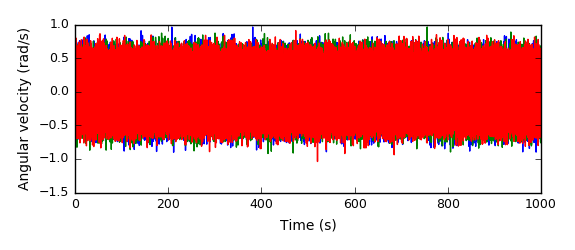
\includegraphics[width=0.7\linewidth]{Figures/noise}
	\caption{Module output of noise standard deviation check.}
	\label{fig:noise}
\end{figure}

\begin{figure}
	\centering
	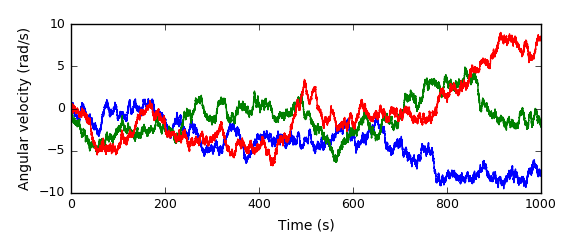
\includegraphics[width=0.7\linewidth]{Figures/walk}
	\caption{Module output for random walk bounds check.}
	\label{fig:walk}
\end{figure}


\end{document}
